\chapter{Building Mental Models}\label{s:models}

\begin{objectives}

\item Explain the cognitive differences between novices and competent
  practitioners in terms of mental models, and the implications of
  these differences for teaching.

\item Define and differentiate formative and summative assessment.

\item Construct multiple-choice questions with plausible distractors
  that have diagnostic power.

\end{objectives}

The first task in teaching is to figure out who your learners are and
what they already know.  Our approach is based on the work of
researchers like Patricia Benner, who studied how nurses progress from
being novices to being experts \cite{Benn2000}. Benner identified five
stages of cognitive development that most people go through in a
fairly consistent way. (We say ``most'' and ``fairly'' because human
beings are highly variable; obsessing over how a few geniuses taught
or learned isn't generally useful.)

For our purposes, we can simplify Benner's progression to three
stages:

\begin{description}

  \item[\glossref{g:novice}{Novices}] don't know what they don't know,
    i.e., they don't yet have a usable mental model of the problem
    domain.  As a result, they reason by analogy and guesswork,
    borrowing bits and pieces of mental models from other domains that
    seem superficially similar.

  \item[\glossref{g:competent-practitioner}{Competent practitioners}]
    can do normal tasks with normal effort under normal circumstances
    because they have a mental model that's good enough for everyday
    purposes.  That model doesn't have to be complete or accurate,
    just useful.

  \item[\glossref{g:expert}{Experts}] have mental models that include
    the complexities and special cases that competent practitioners'
    do not.  This allows experts to handle situations that are out of
    the ordinary, diagnose the causes of problems, and so on.  Like
    competent practitioners, experts know what they don't know and how
    to learn it; we will discuss expertise in more detail in
    \chapref{s:memory}.

\end{description}

So what \emph{is} a \glossref{g:mental-model}{mental model}? As you
may have gathered from the way we used the term above, it is a
simplified representation of the most important parts of some problem
domain that is good enough to enable problem solving.  One example is
the ball-and-spring models of molecules used in high school chemistry.
Atoms aren't actually balls, and their bonds aren't actually springs,
but the model does a good job of helping people reason about chemical
compounds and their reactions. A more sophisticated model of an atom
has a small central ball (the nucleus) surrounded by orbiting
electrons. Again, it's wrong, but useful.

One sign that someone is a novice is that the things they say are
\href{https://en.wikipedia.org/wiki/Not_even_wrong}{not even wrong},
e.g., they think there's a difference between programs they type in
character by character and identical ones that they have copied and
pasted. As \chapref{s:motivation} explains, it is very important not
to make novices uncomfortable for doing this: until they have a better
mental model, reasoning by (inappropriate) borrowing from their
knowledge of other subjects is the best they can do.
  
Presenting novices with a pile of facts is counter-productive, because
they don't yet have a model to fit those facts into.  In fact,
presenting too many facts too soon can actually reinforce the
incorrect mental model they've cobbled together---as \cite{Mull2007a}
observed in a study of video instruction for science students:

\begin{quote}

  Students have existing ideas about{\ldots}phenomena before viewing a
  video. If the video presents{\ldots}concepts in a clear, well
  illustrated way, students believe they are learning but they do not
  engage with the media on a deep enough level to realize that what
  was is presented differs from their prior knowledge{\ldots} There is
  hope, however. Presenting students' common misconceptions in a video
  alongside the{\ldots}concepts has been shown to increase learning by
  increasing the amount of mental effort students expend while
  watching it.

\end{quote}

Your goal when teaching novices should therefore be \emph{to help them
  construct a mental model} so that they have somewhere to put facts.
For example, Software Carpentry's
\href{http://swcarpentry.github.io/shell-novice/}{lesson on the Unix
  shell} introduces fifteen commands in three hours. That's one
command every twelve minutes, which seems glacially slow until you
realize that the lesson's real purpose isn't to teach those fifteen
commands: it's to teach paths, history, tab completion, wildcards,
pipes, command-line arguments, and redirection.  Until novices
understand those concepts, the commands don't make sense; once they do
understand those concepts, they can quickly assemble a repertoire of
commands.

The cognitive differences between novices and competent practitioners
underpin the differences between two kinds of teaching materials. A
tutorial's purpose is to help newcomers to a field build a mental
model; a manual's role, on the other hand, is to help competent
practitioners fill in the gaps in their knowledge.  Tutorials
frustrate competent practitioners because they move too slowly and say
things that are obvious (though they are anything \emph{but} obvious
to novices). Equally, manuals frustrate novices because they use
jargon and \emph{don't} explain things.  This phenomenon is called the
\glossref{g:expertise-reversal}{expertise reversal effect}
\cite{Kaly2003}, and is another reason you have to decide early on who
your lessons are meant for.

\begin{callout}{A Handful of Exceptions}

  One of the reasons Unix and C became popular is that Kernighan et
  al's trilogy \cite{Kern1978,Kern1983,Kern1988} somehow managed to be
  good tutorials \emph{and} good manuals at the same time.  Ray and
  Ray's book on Unix \cite{Ray2014} and Fehily's introduction to SQL
  \cite{Fehi2008} are among the very few other books in computing that
  have accomplished this; even after re-reading them several times, I
  don't know how they manage to do it.

\end{callout}

\section{Are People Learning?}\label{s:models-formative-assessment}

One of the exercises in building a mental model is to clear away
things that \emph{don't} belong. As Mark Twain said, ``It ain't what
you don't know that gets you into trouble. It's what you know for sure
that just ain't so.''  Broadly speaking, novices' misconceptions fall
into three categories:

\begin{description}

  \item[Factual errors] like believing that Vancouver is the
    capital of British Columbia (it's Victoria). These are simple to
    correct, but getting the facts right is not enough on its own.

  \item[Broken models] like believing that motion and acceleration
    must be in the same direction. We can address these by having
    novices reason through examples that draw attention to
    contradictions.

  \item[Fundamental beliefs] such as ``the world is only a few
    thousand years old'' or ``some kinds of people are just naturally
    better at programming than others''
    \cite{Guzd2015b,Pati2016}. These are also broken models, but often
    deeply connected to the learner's social identity, so they resist
    evidence and reason.

\end{description}

Teaching is most effective when teachers identify and clear up
learners' misconceptions \emph{during the lesson}.  This is called
\glossref{g:formative-assessment}{formative assessment}; the word
``formative'' means it is used to form or shape the teaching.
Learners don't pass or fail formative assessment; instead, it tells
the teacher and the learner how they are both doing and what they
should focus on next. For example, a music teacher might ask a learner
to play a scale very slowly in order to see if she is breathing
correctly, while someone teaching web design could ask a learner to
resize the images in a page to check if his explanation of CSS made
sense.

The counterpoint to formative assessment is
\glossref{g:summative-assessment}{summative assessment}, which you do
at the end of the lesson to determine if your teaching was successful,
i.e., whether the learner has understood what you have taught and is
ready to move on.  One way of thinking about the difference is that a
chef tasting food as she cooks it is formative assessments, but the
guests tasting it once it's served is summative.

In order to be useful during teaching, a formative assessment has to
be quick to administer (so that it doesn't break the flow of the
lesson) and give a clear result (so that it can be used with groups as
well as individuals). The most widely used kind of formative
assessment is probably the multiple choice question (MCQ).  A lot of
teachers have a low opinion of them, but when they are designed well,
they can reveal much more than just whether someone knows specific
facts.  For example, suppose you are teaching children how to do
multi-digit addition \cite{Ojos2015}, and you give them this MCQ:

\begin{quote}

  What is 37 + 15? \\
  a) 52 \\
  b) 42 \\
  c) 412 \\
  d) 43

\end{quote}

\noindent
The correct answer is 52, but the other answers provide valuable
insights:

\begin{itemize}

\item
  If the child chooses 42, she is throwing away the carry completely.

\item
  If she chooses 412, she is treating each column of numbers as a
  separate problem unconnected to its neighbors.

\item
  If she chooses 43 then she knows she has to carry the 1, but is
  carrying it back into the column it came from.

\end{itemize}

Each of these incorrect answers is a
\glossref{g:plausible-distractor}{plausible distractor} with
\glossref{g:diagnostic-power}{diagnostic power}.  A distractor is a
wrong or less-than-best answer; ``plausible'' means that it looks like
it could be right, while ``diagnostic power'' means that each of the
distractors helps us figure out what to explain next to that
particular learner.

In order to come up with plausible distractors, think about the
questions your learners asked or problems they had the last time you
taught this subject.  If you haven't taught it before, think about
your own misconceptions, ask colleagues about their experiences, or
look at the history of your field---if everyone misunderstood your
subject in some way fifty years ago, the odds are that a lot of your
learners will still misunderstand it that way today. You can also ask
open-ended questions in class to collect misconceptions about material
to be covered in a later class, or check question and answer sites
like \href{http://www.quora.com}{Quora} or
\href{http://stackoverflow.com}{Stack Overflow} to see what people
learning the subject elsewhere are confused by.

MCQs aren't the only kind of formative assessment you can use: Parsons
Problems (\chapref{s:load}) and matching problems
(\secref{s:exercises-diagrams}) are also quick and unambiguous.
Short-answer questions are another option: if answers are 2--5 words
long, there are few enough plausible answers to make scalable
assessment possible \cite{Mill2016a}.

Developing formative assessment is useful even if you don't use them
in class because it forces you to think about your learners' mental
models and how they might be broken---in short, to put yourself into
your learners' heads and see the topic from their point of view.
Whatever you pick, you should use something that takes a minute or two
every 10--15 minutes to make sure that your learners are actually
learning.  That way, if a significant number of people have fallen
behind, only a short portion of the lesson will have to be repeated.
This rhythm isn't based on an intrinsic attentional limit:
\cite{Wils2007} found little support for the often-repeated claim that
students can only pay attention for 10--15 minutes.  If you are
teaching online (\chapref{s:online}), you should check in much more
often to keep learners engaged.

Formative assessments can also be used preemptively: if you start a
class with an MCQ and everyone answers it correctly, you can skip the
part of the lecture that was going to explain something your learners
already know.  Doing this also shows learners that you respect your
learners' time enough not to waste it, which helps with motivation
(\chapref{s:motivation}).

If the majority of the class chooses the same wrong answer, you should
go back and work on correcting the misconception that distractor
points to.  If their answers are pretty evenly split between several
options they are probably just guessing, so you should back up and
re-explain the idea in a different way.

What if most of the class votes for the right answer, but a few vote
for wrong ones?  In that case, you have to decide whether you should
spend time getting the minority caught up, or whether it's more
important to keep the majority engaged.  No matter how hard you work
or what teaching practices you use, you won't always be able to give
everyone what they need; it's your responsibility as a teacher to make
the call.

\begin{callout}{Concept Inventories}

  Given enough data, MCQs can be made surprisingly precise. The
  best-known example is the Force Concept Inventory \cite{Hest1992},
  which assesses understanding of basic Newtonian mechanics. By
  interviewing a large number of respondents, correlating their
  misconceptions with patterns of right and wrong answers, and then
  improving the questions, its creators constructed a diagnostic tool
  that can pinpoint specific misconceptions.  Researchers can then use
  that tool to measure how effective changes in teaching methods are
  \cite{Hake1998}.

  Tew and others developed and validated a language-independent
  assessment for introductory programming \cite{Tew2011};
  \cite{Park2016} has replicated it, and \cite{Hamo2017} is developing
  a concept inventory for recursion. However, it's very costly to
  build tools like this, and students' ability to search for answers
  online is an ever-increasing threat to their validity.

\end{callout}

Working formative assessments into class requires only a little bit of
preparation and practice.  Giving students colored or numbered cards
so that they can all answer an MCQ at once (rather than holding up
their hands in turn), having one of the options be, ``I have no
idea'', and encouraging them to talk to their neighbors for a few
seconds before answering will all help ensure that your teaching flow
isn't disrupted.  \secref{s:classroom-peer} describes a powerful,
evidence-based teaching method that builds on these simple ideas.

\begin{callout}{Humor}

  Teachers sometimes put supposedly-silly answers like ``my nose!''
  on MCQs, particularly ones intended for younger students. However,
  they don't provide any insight into learners' misconceptions, and
  most people don't actually find them funny (especially on
  re-reading).

\end{callout}

A lesson's formative assessments should prepare learners for its
summative assessment: no one should ever encounter a question on an
exam that the teaching did not prepare them for. This doesn't mean you
should never put new kinds of problems on an exam, but if you do, you
should have given learners practice with (and feedback on) tackling
novel problems beforehand.

\section{Exercises}\label{s:models-exercises}

\exercise{Your Mental Models}{think-pair-share}{15}

What is one mental model you use to understand your work?  Write a few
sentences describing it, and give feedback on a partner's.  Once you
have done that, have a few people share their models with the whole
group.  Does everyone agree on what a mental model is?  Is it possible
to give a precise definition, or is the concept useful precisely
because it is a bit fuzzy?

\exercise{Symptoms of Being a Novice}{whole class}{5}

What are the symptoms of being a novice? I.e., what does someone do or
say that leads you to classify them as a novice in some domain?

\exercise{Modelling Novice Mental Models}{pairs}{20}

Create a multiple choice question related to a topic you have taught
or intend to teach and explain the diagnostic power of each its
distractors (i.e., explain what misconception each distractor is meant
to identify).

When you are done, trade MCQs with a partner.  Is their question
ambiguous?  Are the misconceptions plausible?  Do the distractors
actually test for them?  Are any likely misconceptions \emph{not}
tested for?

\exercise{Other Kinds of Formative Assessment}{whole class}{20}

A good formative assessment requires people to think through a
problem.  For example, imagine that you have placed a block of ice in
a bathtub and then filled the tub to the rim with water.  When the ice
melts, does the water level go up (so that the tub overflows), go
down, or stay the same (\figref{f:models-bathtub})?

\begin{figure}
\centering
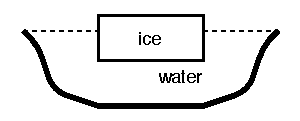
\includegraphics{../docs/fig/bathtub.pdf}
\caption{Ice in a Bathtub}
\label{f:models-bathtub}
\end{figure}

The correct answer is that the level stays the same: the ice displaces
its own weight in water, so it exactly fills the ``hole'' it has made
when it melts. Figuring out why helps people build a model of the
relationship between weight, volume, and density \cite{Epst2002}.

Describe another kind of formative assessment you have seen or used and
explain how it helps both the instructor and the learner figure out
where they are and what they need to do next.

\exercise{A Different Progression}{individual}{15}

The model of skill development described at the start of this chapter
is sometimes called the
\href{https://en.wikipedia.org/wiki/Dreyfus_model\_of\_skill\_acquisition}{Dreyfus
  model}.  Another commonly-used progression is the
\href{https://en.wikipedia.org/wiki/Four_stages_of_competence}{four
  stages of competence}:

\begin{description}

  \item[Unconscious incompetence:] the person doesn't know what they
    don't know.

  \item[Conscious incompetence:] the person realizes that they don't
    know something.

  \item[Conscious competence:] the person has learned how to do
    something, but can only do it while concentrating, and may still
    need to break things down into steps.

  \item[Unconscious competence:] the skill has become second nature,
    and the person can do it reflexively.

\end{description}

\noindent
Identify one subject where you are at each level.  What level are most
of your learners at?  What level are you trying to get them to?

\exercise{What Kind of Book Is This?}{small groups}{5}

What are the chapters in the main body of this book: a tutorial or a
manual?  What about the appendices?  Why?

\exercise{What Kind of Computing?}{individual}{10}

\cite{Tedr2008} summarizes three traditions in computing:

\begin{description}

\item[Mathematical:] Programs are the embodiment of algorithms; they
  are either correct or incorrect, as well as more or less efficient.

\item[Scientific:] Programs are more or less accurate models of
  information processes that can be studied using the scientific
  method.

\item[Engineering:] Programs are built objects like dams and
  airplanes, and are more or less effective and reliable.

\end{description}

\noindent
Which of these best matches your mental model of computing?  If none
of them do, what model do you have?
